\documentclass[12pt, a4paper]{article}

% --- Pacotes Básicos ---
\usepackage{array}
\usepackage[utf8]{inputenc}
\usepackage[T1]{fontenc}
\usepackage[main=brazilian, english]{babel}
\usepackage{indentfirst}
\usepackage[ ]{graphicx}
\usepackage{geometry}
\geometry{left=3cm, top=3cm, right=2cm, bottom=2cm}
\usepackage{booktabs}

% --- Informações do Documento ---
\title{Universidade Federal da Fronteira Sul\\
Relatório Construção de um Analisador Sintático}
\author{Erickson Giesel Müller}
\date{\today}

\begin{document}
\maketitle
\thispagestyle{empty} % primeira página não tem número.
%\newpage

\section{Resumo}
	Este relatório descreve o desenvolvimento e a implementação da primeira etapa de um analisador sintático. O objetivo principal do trabalho consiste em validar a estrutura gramatical de um código-fonte a partir de uma Gramática Livre de Contexto (GLC). A metodologia adotada envolveu a construção de um algoritmo na linguagem Python baseado na abordagem de análise ascendente, integrado à fita de saída de um analisador léxico. O sistema implementado realiza a leitura dinâmica da gramática, aplica algoritmos de tratamento para a eliminação de símbolos inúteis e fatoração, e calcula os conjuntos matemáticos FIRST e FOLLOW. Para o motor de reconhecimento, utiliza-se uma tabela de parsing SLR consumida por um autômato com pilha. Os resultados demonstram que o analisador é capaz de processar os tokens, aceitando estruturas válidas da linguagem e emitindo diagnósticos precisos de erros sintáticos ao interceptar anomalias na fita, cumprindo todos os requisitos exigidos para a fase de análise sintática.

\section{Introdução}
	No processo de construção de um compilador, a tradução de um código-fonte para uma linguagem de máquina ou intermediária é dividida em diversas fases lógicas. Enquanto a análise léxica atua como a primeira linha de processamento, agrupando caracteres em unidades com significado, chamados de tokens, é a análise sintática que assume a responsabilidade de validar se a disposição desses tokens obedece às regras estruturais da linguagem projetada.

	Este relatório documenta o desenvolvimento da etapa de análise sintática de um compilador. O projeto tem como escopo a implementação de um analisador sintático, projetado para consumir a fita de saída do analisador léxico desenvolvido no trabalho 1. O analisador valida as cadeias de entrada contra uma Gramática Livre de Contexto utilizando uma tabela de parsing da classe SLR. O código foi desenvolvido na linguagem Python e abrange algoritmos como a eliminação de símbolos inúteis, fatoração de regras para remoção de ambiguidades e a construção dos conjuntos matemáticos FIRST e FOLLOW.

	%Para apresentar o desenvolvimento desta ferramenta, o presente relatório está estruturado da seguinte forma: a Seção 2 apresenta o Referencial Teórico, abordando os conceitos fundamentais de gramáticas e autômatos com pilha; a Seção 3 detalha a Implementação e os Resultados, demonstrando o funcionamento dos algoritmos e a eficácia do motor Shift-Reduce frente a fitas de tokens; por fim, a Seção 4 expõe as Conclusões extraídas durante o desenvolvimento do projeto.

\section{Referencial Teórico}
	%A função carregar_glc(self, caminho_arquivo) lê esse arquivo de texto e o converte dinamicamente para o dicionário self.glc na memória, mapeando os Não-Terminais para as suas respectivas listas de produções.
	%A função eliminar_inuteis(self) divide o processo em duas fases (encontrar geradores e alcançar a partir do Símbolo Inicial).
	%A função fatorar_glc(self) procura prefixos em comum e cria novos estados para remover o não-determinismo.
	%FIRST e FOLLOW: Estão implementados e calculados pelas funções first(self, term), first_seq(self, rhs, first_dict) e follow(self). Os resultados são salvos em self.first_sets e self.follow_sets.

	A análise sintática é a segunda fase do processo de compilação, responsável por verificar se a estrutura dos tokens gerados pelo analisador léxico está de acordo com as regras formais da linguagem. Para descrever a sintaxe de linguagens de programação, utilizam-se as Gramáticas Livres de Contexto (GLC).

	Uma GLC é formalmente definida por um conjunto de variáveis (ou Não-Terminais), um conjunto de símbolos terminais (tokens), um conjunto de regras de produção e um símbolo inicial. No escopo deste projeto, a representação computacional da gramática é inicializada pela função \texttt{carregar\_glc(self, caminho\_arquivo)}. Este método lê o arquivo de texto contendo as regras de produção e o converte dinamicamente para a estrutura de dicionário \texttt{self.glc} na memória do programa, mapeando os Não-Terminais para as suas respectivas listas de derivações.

	\subsection{Tratamento da Gramática}

--- GLC Final Pós-Processamento ---\\
<PROGRAMA> -> [['<DECLARACAO>'], ['<PROGRAMA>', '<DECLARACAO>']]\\
<DECLARACAO> -> [['definir', 'variavel', 'como', 'tipo', 'string'], ['<tipo>', 'variavel', '=', 'new', '<classe>']]\\

Terminais detectados: {'<tipo>', 'como', 'variavel', 'tipo', 'definir', 'new', 'string', '=', '<classe>'}\\
	Para que uma gramática seja adequadamente processada por um autômato (especialmente em abordagens tabulares), ela frequentemente precisa passar por transformações estruturais que garantam seu determinismo e validade.

	O primeiro passo consiste na eliminação de símbolos inúteis, que são variáveis que nunca geram uma cadeia de terminais (não-geradores) ou que nunca podem ser alcançadas a partir do símbolo inicial (incessíveis). O algoritmo implementado na função \texttt{eliminar\_inuteis(self)} atua dividindo este processamento exatamente nessas duas fases: primeiramente, varre a gramática para encontrar e preservar apenas os símbolos geradores; em seguida, realiza uma travessia a partir do símbolo inicial para reter apenas os símbolos alcançáveis.

	O segundo tratamento aplicado é a fatoração da GLC. A ambiguidade estrutural surge quando uma gramática possui regras de produção para um mesmo Não-Terminal que iniciam com o mesmo prefixo, exigindo que o analisador tente adivinhar qual caminho seguir. A função \texttt{fatorar\_glc(self)} resolve este não-determinismo procurando prefixos em comum nas opções de derivação. Ao encontrar repetições, o algoritmo isola o prefixo e cria novos estados artificiais para derivar os sufixos restantes.

	\subsection{Conjuntos FIRST e FOLLOW}
	O núcleo matemático preditivo de um analisador sintático baseia-se nos conjuntos FIRST e FOLLOW. O conjunto $FIRST(\alpha)$ agrupa os símbolos terminais que iniciam as cadeias derivadas a partir da sequência $\alpha$. Já o conjunto $FOLLOW(A)$ agrupa os terminais que podem aparecer imediatamente à direita do Não-Terminal $A$ em alguma forma sentencial válida.

	No sistema desenvolvido, esses conjuntos formam a base para o reconhecimento das transições de estados. Eles estão puramente implementados e são calculados de forma iterativa pelas funções \texttt{first(self, term)}, pela função auxiliar \texttt{first\_seq(self, rhs, first\_dict)} que é responsável por tratar a propagação da palavra vazia ($\varepsilon$) ao longo da cadeia e pela função \texttt{follow(self)}. Para garantir a eficiência de acesso durante o consumo da fita pelo motor de reconhecimento, os resultados computados são salvos definitivamente nas variáveis de instância \texttt{self.first\_sets} e \texttt{self.follow\_sets}.

	\subsection{Tabela de Parsing SLR e Algoritmo de Mapeamento}
	Os analisadores sintáticos ascendentes (Bottom-Up) constroem a árvore de derivação a partir das folhas (tokens) em direção à raiz (símbolo inicial). Para gerenciar essa construção, utiliza-se um Autômato com Pilha guiado por uma Tabela de Parsing, sendo a classe SLR (Simple LR) uma das mais eficientes de se implementar.

	A tabela SLR é dividida em duas partes: a função ACTION, que determina a ação a ser tomada com base no estado atual e no token lido; e a função GOTO, que dita o próximo estado após uma redução. As operações principais da máquina de estados são o \textit{Shift} (empilhar o token e transitar para um novo estado) e o \textit{Reduce} (substituir um corpo de regra pelo seu Não-Terminal correspondente, desempilhando os estados anteriores).

	No projeto, a estrutura dessa matriz matemática foi carregada pela função \texttt{carregar\_tabela\_slr(self)}. Já a implementação do algoritmo de mapeamento que consome a fita de entrada encontra-se na função \texttt{executar\_parser(self)}. Este algoritmo controla um laço de repetição acoplado a uma lista que simula a pilha (\texttt{pilha = [0]}), consultando iterativamente a tabela para aceitar a cadeia (\texttt{acc}) ou emitir um diagnóstico de erro sintático ao encontrar um cruzamento vazio.

	\begin{center}
	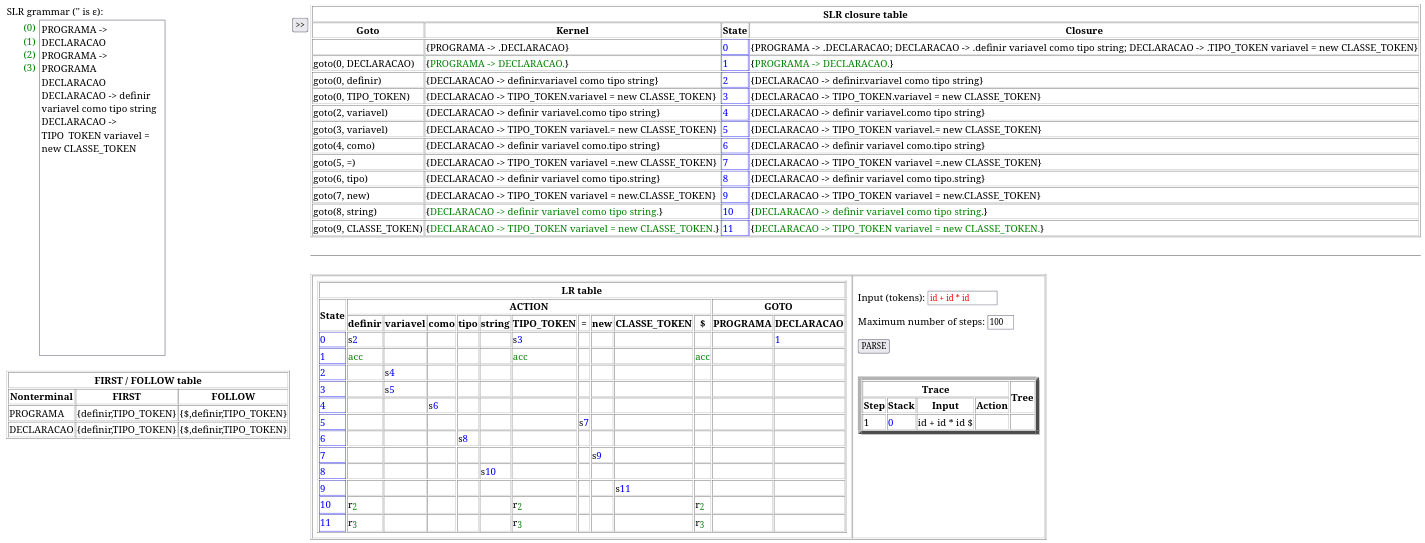
\includegraphics[scale=0.4]{images/slr.png}\\
		\textit{Fonte: SLR Parser Generator}
	\end{center}

	\subsection{Tabela de Símbolos}
	A Tabela de Símbolos é uma estrutura de dados fundamental que permeia todas as fases da compilação. Seu papel é armazenar informações sobre os identificadores e tokens encontrados no código-fonte, servindo como a principal via de comunicação entre o analisador léxico, o sintático e as futuras fases de análise semântica e geração de código.

	No escopo desta implementação, a tabela é inicialmente construída e populada durante a fase léxica (armazenando linha, identificador, rótulo e palavra lida) e injetada na inicialização da classe \texttt{AnalisadorSintatico} através da variável \texttt{self.tabela\_simbolos}. A arquitetura garante que, durante a operação de \textit{Reduce} no mapeamento sintático, o compilador tenha o contexto estrutural exato para, nas etapas subsequentes, adicionar propriedades semânticas (como escopo e tipo de dado) a esta mesma tabela.

\section{Implementação e Resultados}
	
	Considerando que o algoritmo usou os seguintes tokens e gramática em \texttt{fonte.txt}:
\begin{verbatim}
definir
como
tipo
string

S::=a<A>|e<A>|i<A>|o<A>|u<A>|C<A>|T<A>|F<A>|G<A>|R<A>
A::=f<A>|a<A>|e<A>|i<A>|{epsilon}
\end{verbatim}
	Realizaram-se os testes de sucesso e erro sintáticos com os seguintes códigos:
	\begin{verbatim}
	definir Teia como tipo string (sucesso)
	definir Xeia como tipo string (erro)
	\end{verbatim}
	Dos quais, o analisador respondeu, respectivamente, os seguintes outputs:
	\begin{center}
		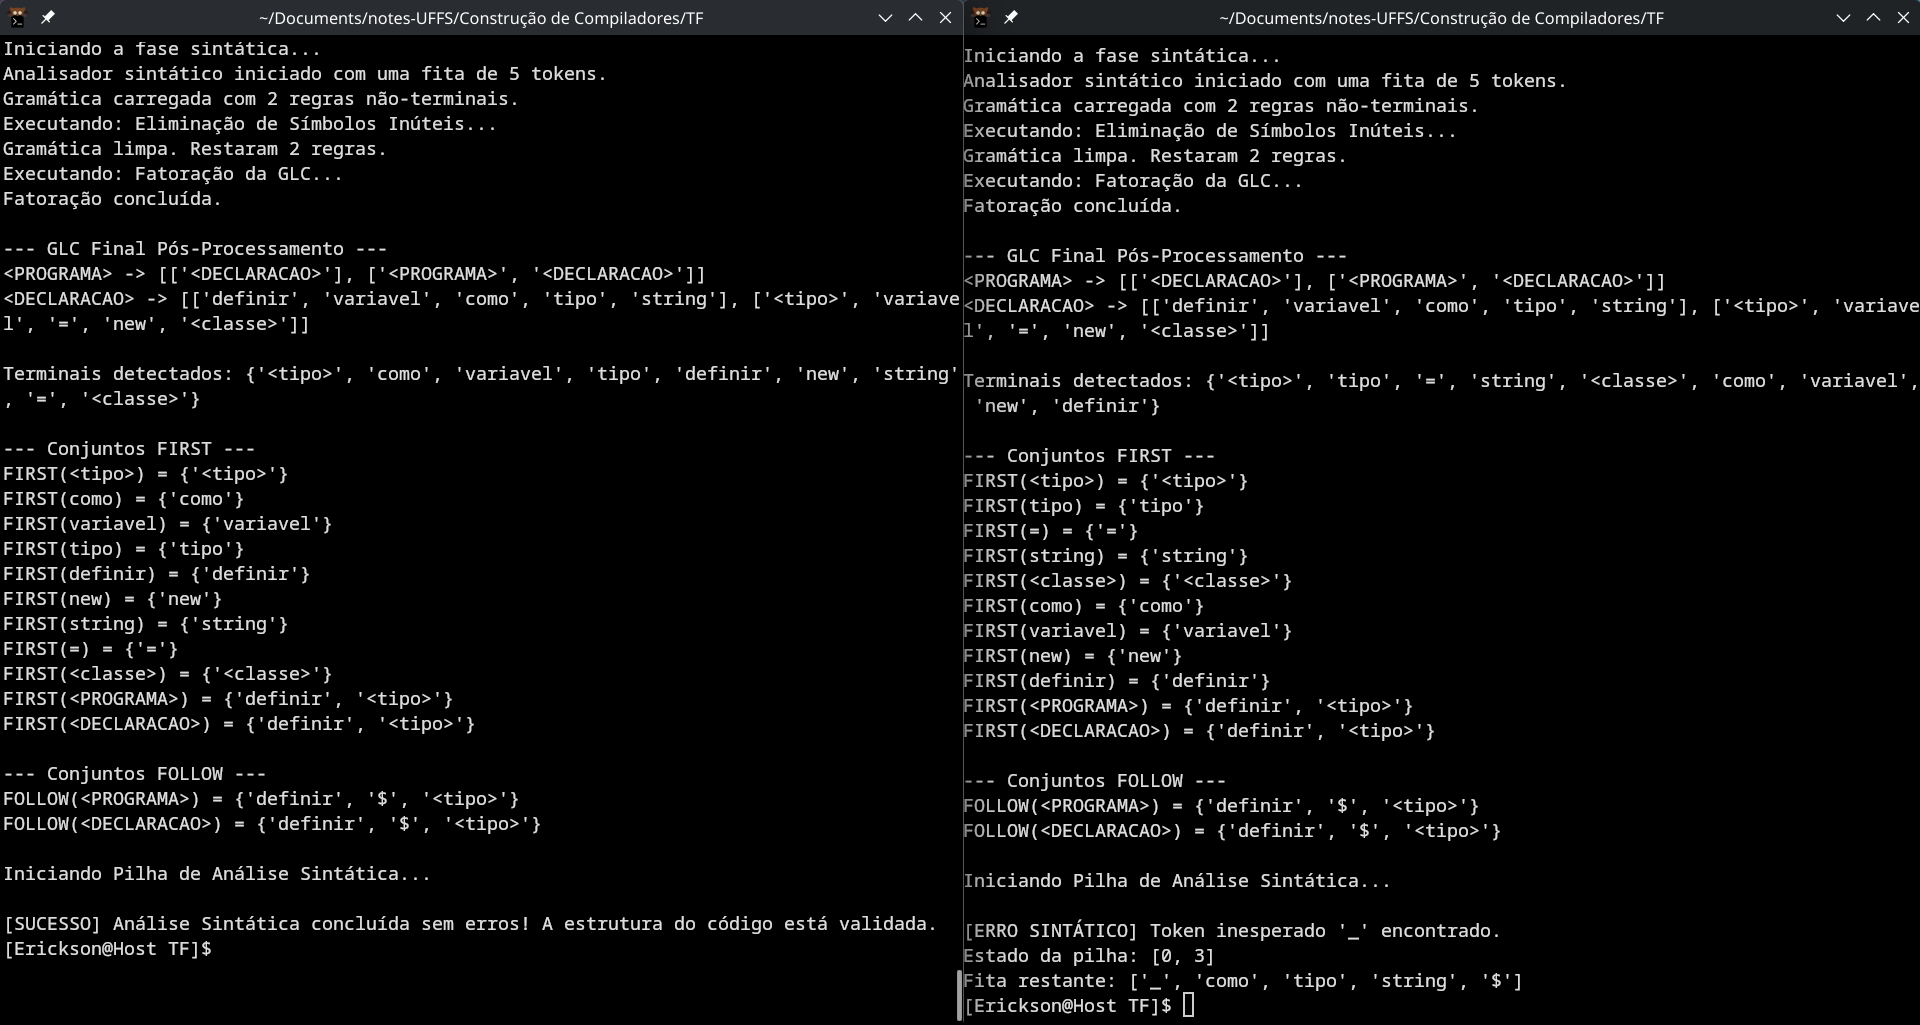
\includegraphics[scale=0.33]{images/teste.png}
	\end{center}
	


\section{Conclusão}
	O desenvolvimento do analisador sintático demonstrou, na prática, a eficácia da integração entre as fases iniciais da construção de um compilador. A implementação rigorosa dos algoritmos de tratamento da Gramática Livre de Contexto (eliminação de símbolos inúteis e fatoração), aliada ao cálculo automatizado dos conjuntos matemáticos FIRST e FOLLOW, forneceu a base formal necessária para o funcionamento do motor de reconhecimento.

	A escolha da abordagem ascendente (Bottom-Up) guiada por uma tabela de parsing SLR provou ser uma arquitetura eficiente. Como evidenciado nos testes práticos, o autômato de pilha operou de maneira previsível, consumindo tokens válidos até o estado de aceitação,  interceptando com precisão as anomalias estruturais e lexicais (bloqueando a execução e emitindo diagnósticos claros sobre o estado da máquina).

	Por fim, a inicialização e o trânsito da Tabela de Símbolos durante o processo de análise sintática deixam a arquitetura do sistema perfeitamente engatilhada para as próximas fases. O compilador encontra-se estruturalmente sólido e pronto para receber a implementação da análise semântica.

\begin{thebibliography}{9}
\bibitem{apostila} SCHEFFEL, Roberto M.
\textit{Apostila Linguagens Formais e Autômatos}.
\bibitem{aho}
AHO, A. V.; LAM, M. S.; SETHI, R.; ULLMAN, J. D. \textbf{Compiladores: princípios, técnicas e ferramentas}. 2. ed. São Paulo: Pearson Education do Brasil, 2007.

\bibitem{louden}
LOUDEN, K. C. \textbf{Compiladores: princípios e práticas}. São Paulo: Thomson Learning, 2004.

\end{thebibliography}

\end{document}
